\documentclass[conference]{IEEEtran}
\IEEEoverridecommandlockouts

\usepackage{cite}
\usepackage{amsmath,amssymb,amsfonts}
\usepackage{graphicx}
\usepackage{textcomp}
\usepackage{xcolor}
\usepackage{float}
\usepackage[utf8]{inputenc}
\usepackage[T1]{fontenc}
\usepackage[spanish]{babel}

\addto\captionsspanish{
  \renewcommand{\abstractname}{Abstract}
  \renewcommand{\IEEEkeywordsname}{Keywords}
}

\def\BibTeX{{\rm B\kern-.05em{\sc i\kern-.025em b}\kern-.08em
    T\kern-.1667em\lower.7ex\hbox{E}\kern-.125emX}}

\begin{document}

\title{De Radiofrecuencia a la Envolvente Compleja con Modulaciones Digitales (GNU Radio)*\\
{\footnotesize \textsuperscript{*}Repositorio: \url{https://github.com/TU_USUARIO/TU_REPO/tree/Practica_4}}}

\author{
\IEEEauthorblockN{1\textsuperscript{st} Nombre Apellido}
\IEEEauthorblockA{\textit{Código: XXXXXXX}\\
\textit{Universidad Industrial de Santander}\\
correo@correo.uis.edu.co}
\and
\IEEEauthorblockN{2\textsuperscript{nd} Nombre Apellido}
\IEEEauthorblockA{\textit{Código: XXXXXXX}\\
\textit{Universidad Industrial de Santander}\\
correo@correo.uis.edu.co}
\and
\IEEEauthorblockN{3\textsuperscript{rd} Nombre Apellido}
\IEEEauthorblockA{\textit{Código: XXXXXXX}\\
\textit{Universidad Industrial de Santander}\\
correo@correo.uis.edu.co}
}

\maketitle

% ============================================================
\begin{abstract}
This paper presents the analysis of digital modulations OOK, BPSK, and FSK in both 
Radio Frequency (RF) and Complex Envelope (CE) representations using GNU Radio 
Companion (GRC). Custom VCO blocks are used to generate each modulation scheme, 
and signals are characterized in the time domain, frequency domain, and IQ 
constellation. Results confirm that FSK is a constant-envelope modulation whose 
CE representation is independent of carrier frequency, exhibiting two spectral 
peaks separated by $2f_d$ and a circular IQ trajectory. The minimum spectral 
overlap condition $f_d \geq R_b/2$ is experimentally verified.
\end{abstract}

\begin{IEEEkeywords}
FSK, OOK, BPSK, complex envelope, GNU Radio, VCO, phase accumulator, constellation.
\end{IEEEkeywords}

% ============================================================
\section{Introducción}

En comunicaciones digitales, la misma señal modulada puede representarse como una 
señal paso-bandas (RF) o mediante su Envolvente Compleja (EC) en banda base. La EC 
simplifica el análisis matemático y los algoritmos de procesamiento, ya que elimina 
la dependencia con la frecuencia portadora $f_c$ \cite{proakis2008}. Esta práctica 
estudia tres esquemas de modulación digital —OOK, BPSK y FSK— en ambas 
representaciones, implementados con bloques VCO personalizados en GNU Radio. 
Los bloques \texttt{e\_RF\_VCO\_ff} y \texttt{e\_CE\_VCO\_fc} generan, 
respectivamente, la señal RF y la señal CE compleja a partir de dos entradas: 
amplitud $A$ (entrada superior) y fase $\theta$ (entrada inferior) \cite{gnuradio}.


\section{Modulación FSK en Versión RF y Envolvente Compleja}
\label{sec:fsk}

\subsection{Metodología}

El flujograma base \texttt{RF\_EC\_ook.grc} fue adaptado y guardado como 
\texttt{RF\_EC\_fsk.grc}. La modulación FSK requiere que la información binaria 
controle la frecuencia instantánea de los VCOs, lo que se logra inyectando una 
fase acumulada en la entrada inferior de los bloques VCO, manteniendo amplitud 
constante $A = 1$ en la entrada superior.

La señal binaria $m[n] \in \{0,1\}$ se convierte a formato bipolar activando los 
bloques \textit{Add Const} ($-0.5$) y \textit{Multiply Const} ($\times 2$):
\begin{equation}
    m_{bp}[n] = 2\bigl(m[n] - 0.5\bigr) \in \{-1,\,+1\}
    \label{eq:bipolar}
\end{equation}
Tras el \textit{Interpolating FIR Filter} ($Sps = 128$), el bloque 
\texttt{e\_Acum} calcula la suma acumulada de $m_{bp}$, y el bloque 
\textit{Multiply Const} la escala con:
\begin{equation}
    k_\phi = \frac{2\pi f_d}{R_b \cdot Sps} \approx 0.04908\;\text{rad/muestra}
    \label{eq:kphi}
\end{equation}
La fase resultante $\theta[n]$ produce las señales:
\begin{equation}
    s_{RF}[n] = \cos\!\Bigl(2\pi f_c \tfrac{n}{f_s} + \theta[n]\Bigr), \quad
    s_{CE}[n] = e^{\,j\,\theta[n]}
    \label{eq:fsk}
\end{equation}
El diagrama de bloques completo del modulador FSK se presenta en la 
Fig.~\ref{fig:bloques_fsk}.


\begin{figure}[H]
    \centering
    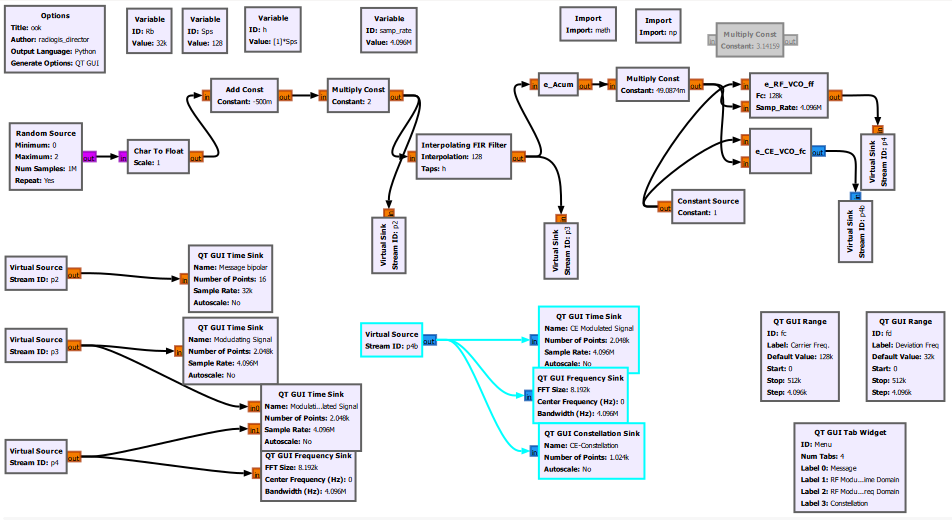
\includegraphics[width=0.48\textwidth]{images/bloques_fsk.png}
    \caption{Diagrama de bloques del modulador FSK en GNU Radio. La señal bipolar 
             pasa por el acumulador de fase y el escalado $k_\phi$ antes de 
             alimentar la entrada de fase de los VCOs.}
    \label{fig:bloques_fsk}
\end{figure}

\subsection{Resultados en el dominio del tiempo}

La Fig.~\ref{fig:tiempo_fsk} muestra la señal modulante bipolar superpuesta con 
la señal RF modulada en FSK. Se observan claramente dos frecuencias instantáneas 
distintas: $f_c - f_d$ para el bit ``0'' y $f_c + f_d$ para el bit ``1''.


\begin{figure}[H]
    \centering
    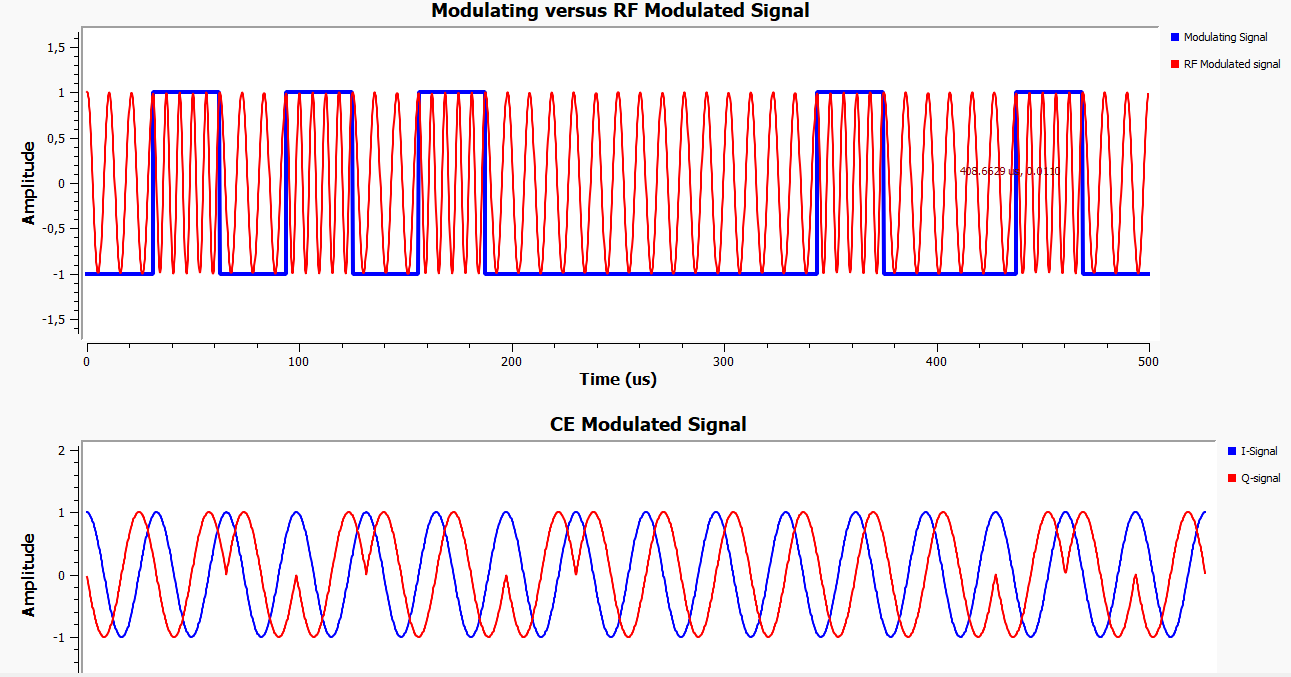
\includegraphics[width=0.48\textwidth]{images/tiempo_fsk.png}
    \caption{Dominio del tiempo: señal modulante bipolar (azul) y señal FSK en RF 
             (rojo) con $f_c=128\,\text{kHz}$, $f_d=32\,\text{kHz}$. Los segmentos 
             de bit ``0'' y ``1'' presentan frecuencias instantáneas $f_c \mp f_d$.}
    \label{fig:tiempo_fsk}
\end{figure}

Al variar $f_c$ con $f_d$ fijo, la densidad de ciclos por símbolo cambia en la 
señal RF pero la EC permanece invariante, lo que confirma que 
$s_{CE}[n] = e^{j\theta[n]}$ no depende de la portadora. Al variar $f_d$ con $f_c$ 
fijo, la diferencia entre las dos frecuencias instantáneas se hace más o menos 
evidente tanto en RF como en la velocidad de rotación del fasor CE.

\subsection{Resultados en el dominio de la frecuencia}

La Fig.~\ref{fig:espectro_fsk} presenta los espectros RF y CE de la señal FSK.


\begin{figure}[H]
    \centering
    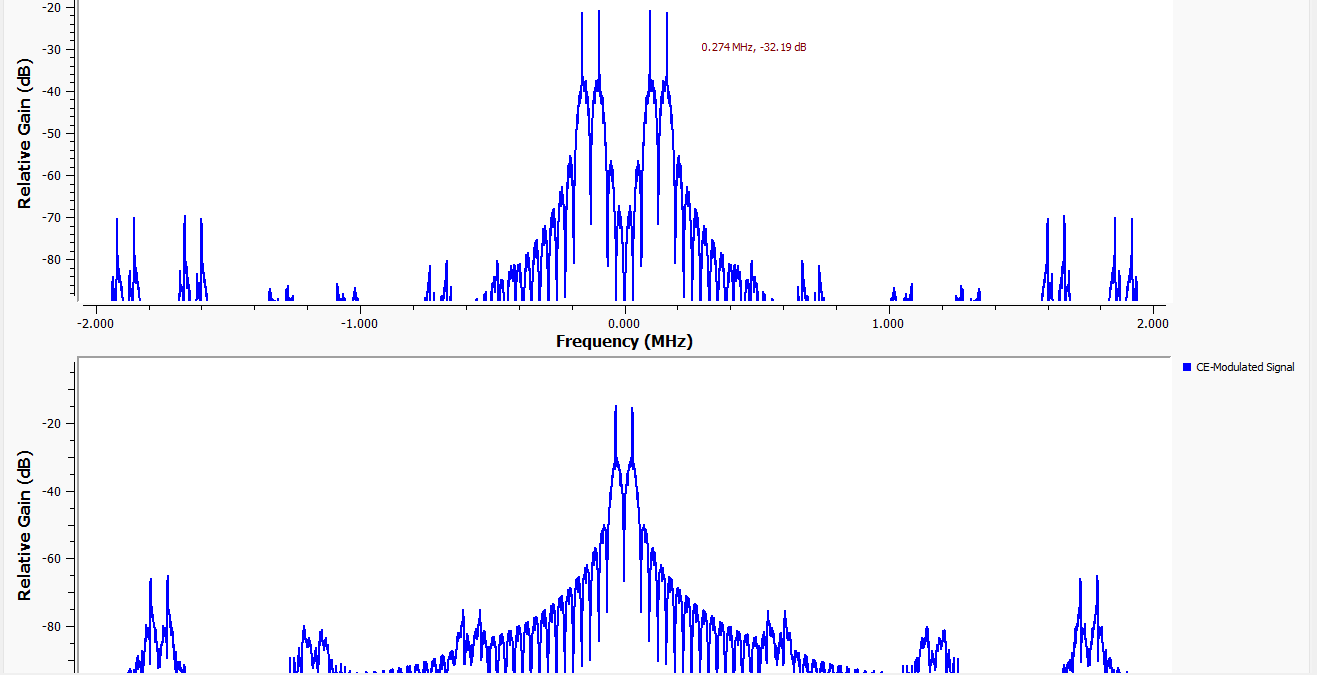
\includegraphics[width=0.48\textwidth]{images/espectro_fsk.png}
    \caption{Espectro de potencia de la señal FSK. \textbf{(a)} Versión RF: picos 
             en $f_c \pm f_d = \{96, 160\}\,\text{kHz}$. \textbf{(b)} Versión CE: 
             picos en $\pm f_d = \pm 32\,\text{kHz}$, independiente de $f_c$.}
    \label{fig:espectro_fsk}
\end{figure}

Para minimizar el solapamiento espectral, la separación entre lóbulos $2f_d$ debe 
superar el ancho del lóbulo principal $\approx 2R_b$, imponiendo la condición de 
ortogonalidad mínima $f_d \geq R_b/2 = 16\,\text{kHz}$. La 
Fig.~\ref{fig:espectro_comp} compara dos configuraciones: $f_d = 8\,\text{kHz}$ 
(solapamiento) y $f_d = 48\,\text{kHz}$ (separación óptima).


\begin{figure}[H]
    \centering
    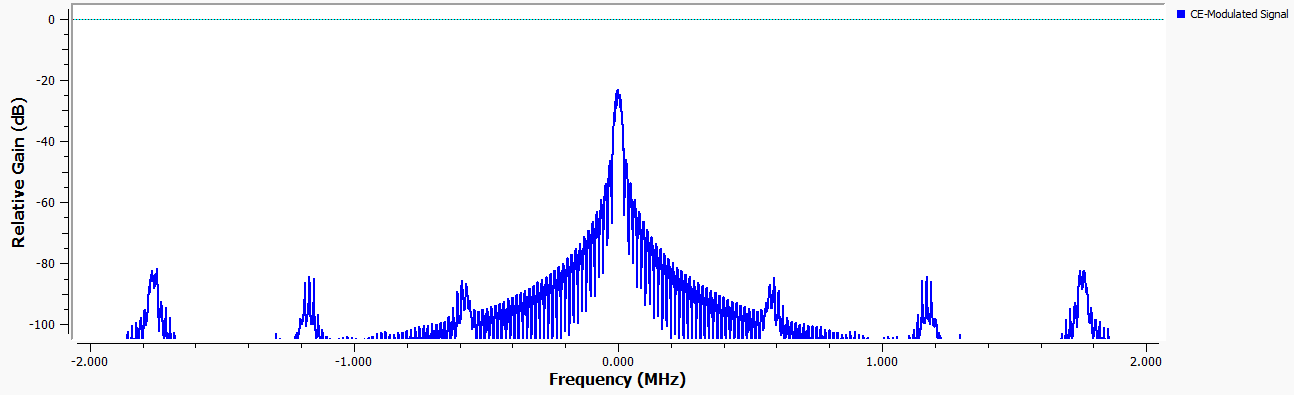
\includegraphics[width=0.23\textwidth]{images/espectro_fd8.png}\hfill
    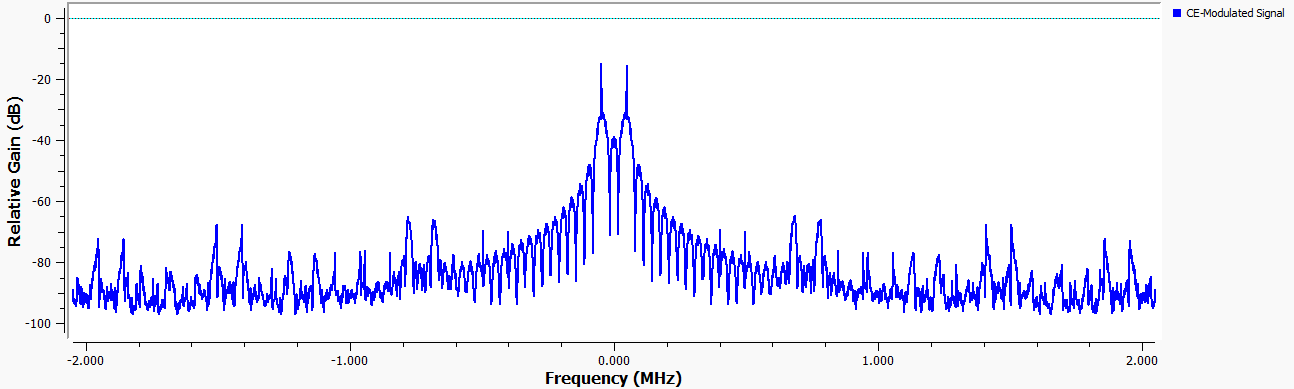
\includegraphics[width=0.23\textwidth]{images/espectro_fd48.png}
    \caption{Espectro CE comparativo. \textbf{Izq.:} $f_d=8\,\text{kHz}$, 
             solapamiento entre lóbulos. \textbf{Der.:} $f_d=48\,\text{kHz}$, 
             separación óptima con mínimo ancho de banda total.}
    \label{fig:espectro_comp}
\end{figure}

\subsection{Constelación IQ de la señal FSK}
\label{subsec:constelacion}

La Fig.~\ref{fig:constelacion_fsk} muestra la constelación IQ de la señal FSK en 
versión CE para dos valores de $f_d$.


\begin{figure}[H]
    \centering
    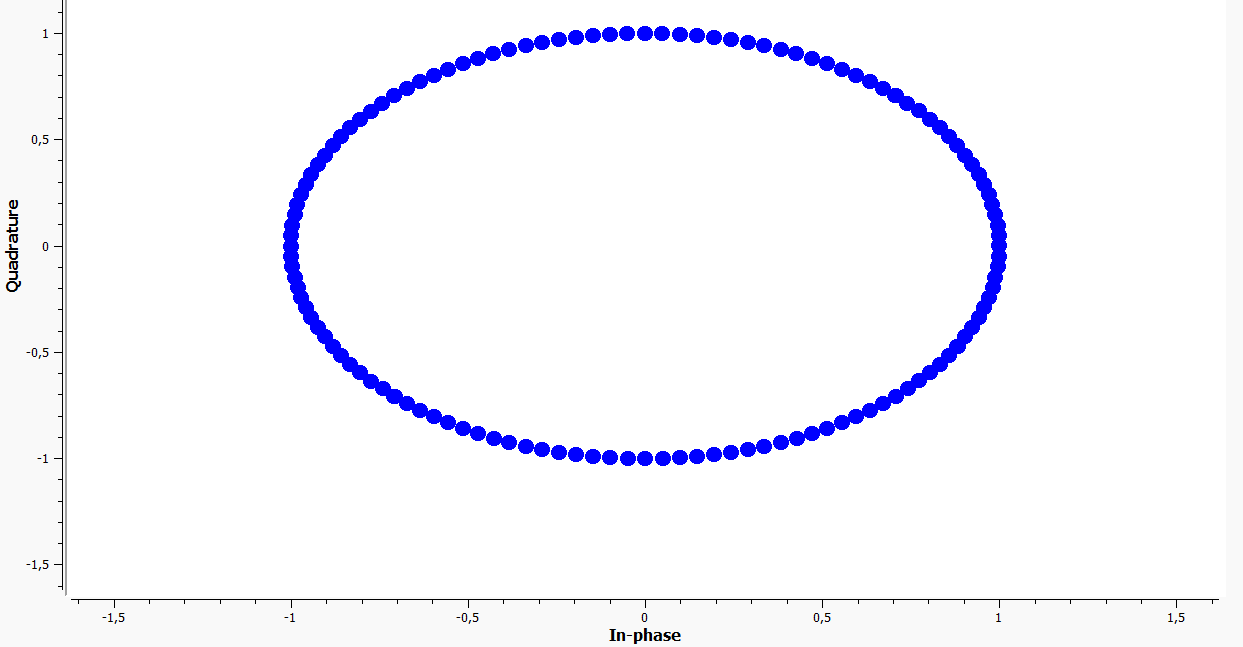
\includegraphics[width=0.23\textwidth]{images/const_fd32.png}\hfill
    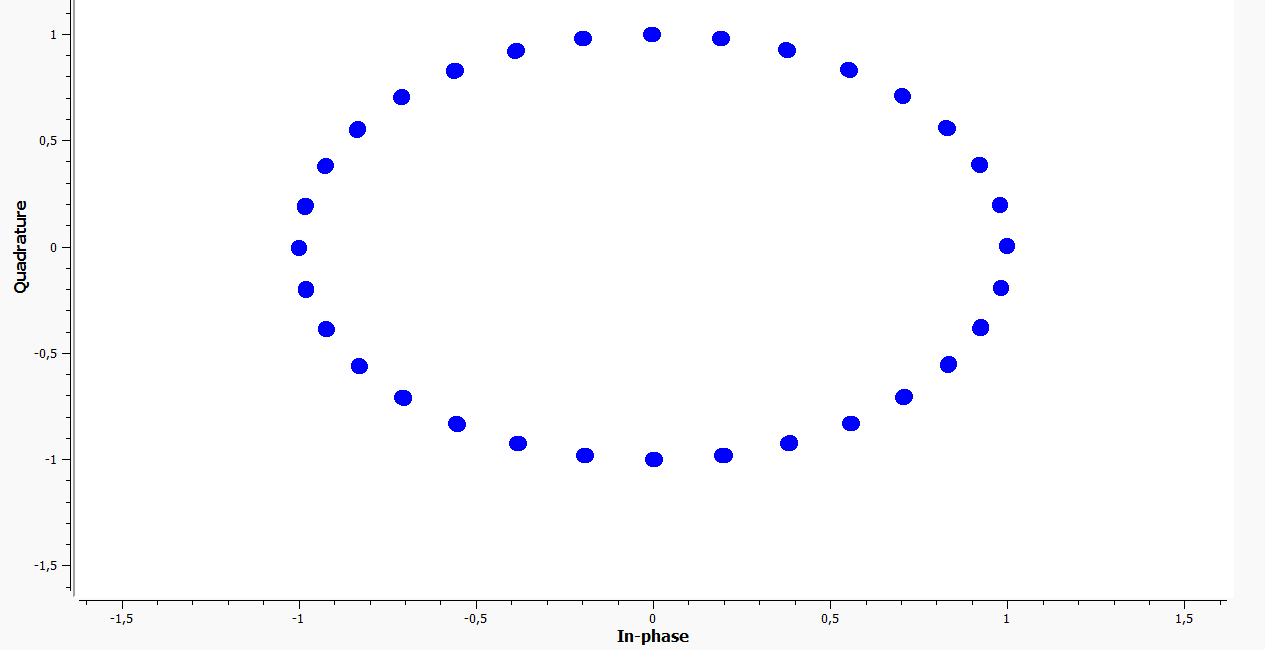
\includegraphics[width=0.23\textwidth]{images/const_fd128.png}
    \caption{Constelación IQ de FSK. \textbf{Izq.:} $f_d=32\,\text{kHz}$, arco 
             sobre la circunferencia unitaria. \textbf{Der.:} $f_d=128\,\text{kHz}$, 
             círculo completo. En ambos casos el módulo $|s_{CE}|=1$.}
    \label{fig:constelacion_fsk}
\end{figure}

Dado que $s_{CE}[n] = e^{j\theta[n]}$ tiene módulo unitario para todo $n$, la 
constelación de FSK siempre describe una trayectoria sobre la circunferencia de 
radio 1. Esto contrasta con BPSK (dos puntos en $\pm 1$) y OOK (dos puntos en 
$0$ y $+1$), y refleja la propiedad de envolvente constante de FSK, que la hace 
robusta frente a amplificadores no lineales \cite{haykin2001}.

% ============================================================
% SECCIÓN DE CONCLUSIONES — completar con aporte de todos los puntos
% ============================================================
\section{Conclusiones}

La implementación de FSK en GNU Radio requiere acondicionar la señal de mensaje 
como fase acumulada antes de los VCOs. La frecuencia portadora $f_c$ no afecta 
la representación EC: el espectro CE permanece centrado en cero y la constelación 
no cambia con variaciones de $f_c$. La condición $f_d \geq R_b/2$ garantiza 
separación espectral mínima, y experimentalmente $f_d = R_b$ ofrece buena 
eficiencia espectral sin solapamiento. La constelación circular de FSK confirma 
su envolvente constante, a diferencia de OOK y BPSK cuyas constelaciones son 
discretas sobre el eje real.

% [Conclusiones de los demás puntos se agregan aquí]

% ============================================================
\begin{thebibliography}{00}

\bibitem{proakis2008}
J. G. Proakis y M. Salehi, \textit{Digital Communications}, 5th~ed.
New York, NY, USA: McGraw-Hill, 2008.

\bibitem{haykin2001}
S. Haykin, \textit{Communication Systems}, 4th~ed.
New York, NY, USA: Wiley, 2001.

\bibitem{gnuradio}
GNU Radio Project, ``GNU Radio Documentation,'' 2024. [En línea].
Disponible en: \url{https://wiki.gnuradio.org}

\end{thebibliography}

\end{document}